\documentclass[a4paper,11pt, twocolumn]{article}
\usepackage[margin=0.8in]{geometry}
\usepackage{xcolor}
\usepackage{graphicx} %package to manage images
\graphicspath{ {./images/} }
\usepackage{amsmath}
\usepackage{amssymb}

\title{A2-6 Digital Communications}
\author{Revision sheet}
\date{}

\usepackage{fancyhdr}
\pagestyle{fancy}
\fancyhead{} % clear all header fields
\renewcommand{\headrulewidth}{0pt} % no line in header area
\fancyfoot{} % clear all footer fields
\renewcommand{\footrulewidth}{0.4pt}
\fancyfoot[C]{\thepage} % page number in centre of the page
\fancyfoot[R]{\footnotesize Thomas Boxall \\ Images from WJEC E-Book} % right hand footer has author name on top line and images reference on bottom line
\fancyfoot[L]{\footnotesize A2-6 Digital Communications \\ Revision sheet} % left hand footer has title of document on top line and 'Revision Sheet' on bottom line


\begin{document}

\maketitle
\thispagestyle{fancy}

% CONTENTS OF THE REVISION SHEET HERE

\section{Shift Registers}
Data can be transmitted either in serial or parallel form. Serial is where you transmit on bit after the other, with the MSB first. Parallel is where all the bits are transmitted simultaneously. Generally, data signals are transmitted in serial.
\subsection{PISO}
The circuit diagram for a \textit{Parallel In Serial Out} shift register is shown below.
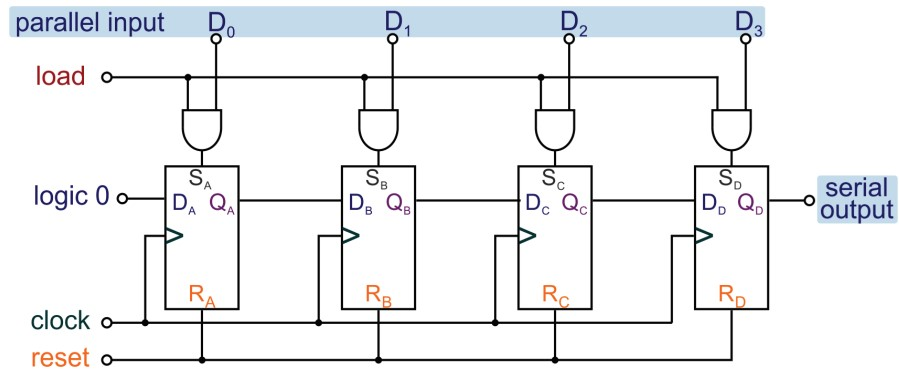
\includegraphics[width=\linewidth]{piso.jpg}
A PISO works as follows
\begin{enumerate}
    \item A logic high pulse is sent to the rest pin - resetting all flip-flops
    \item The 4-bit word is setup on $D_0$ to $D_3$ inputs
    \item The load line is taken high, $D_0$ to $D_3$ is transferred to the flip-flops
    \item Clock is pulsed to shift data out, MSB first
    \item After n-1 pulses, whole word is transmitted
    \item After n pulses the shift register is empty
\end{enumerate}
(where n = number of bits)\\
The progress of bits through the PISO can be displayed in a table.
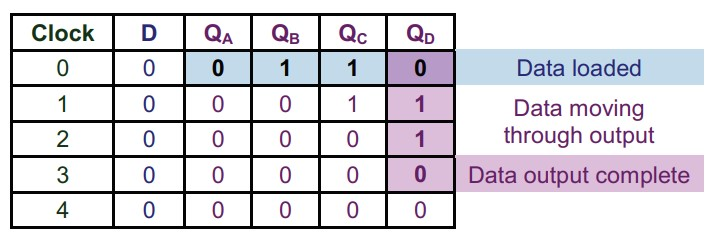
\includegraphics[width=\linewidth]{pisoTable.jpg}
The outputs $Q_A$ to $Q_D$ can be displayed on a timing diagram.
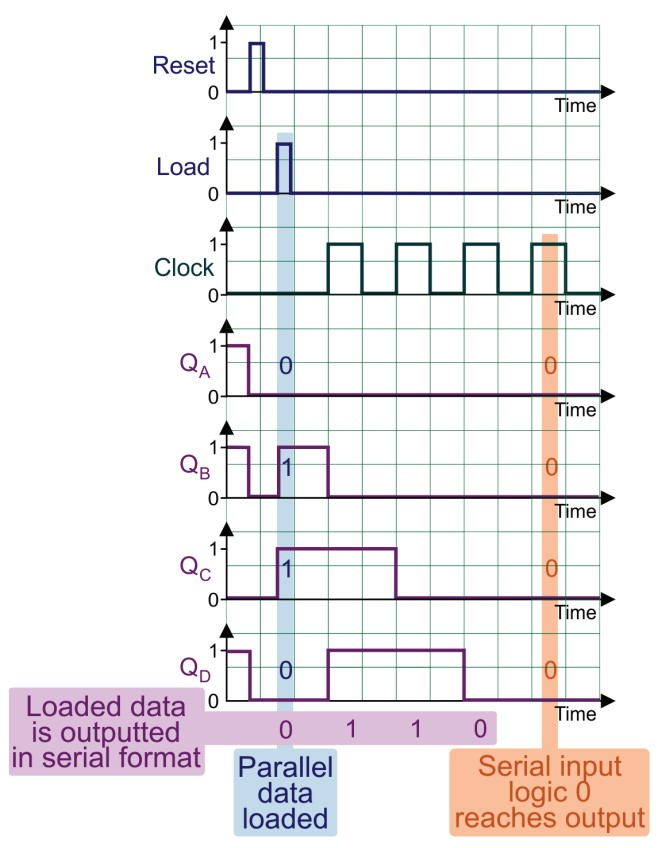
\includegraphics[width=\linewidth]{pisoTiming.jpg}
\subsection{SIPO}
The circuit diagram for a \textit{Serial In Parallel Out} shift register is shown below.
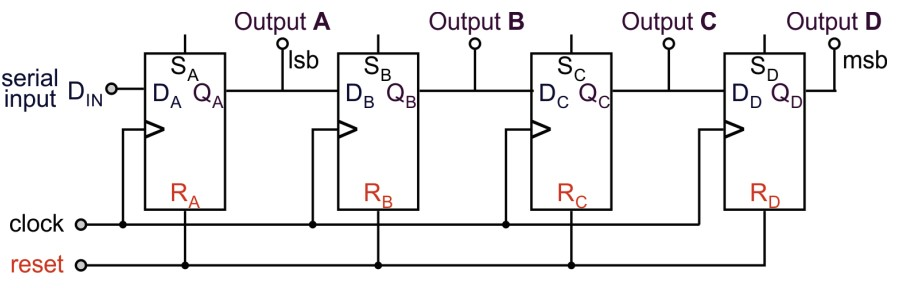
\includegraphics[width=\linewidth]{sipo.jpg}
A SIPO works as follows
\begin{enumerate}
    \item A logic high pulse is sent to the reset pin which resets all the flip-flops
    \item On each clock pulse, the data on input $D_A$ is loaded onto $Q_A$. Each bit is shifted along one
    \item After n pulses, the whole word is received
\end{enumerate}
(where n = number of bits)\\
The progress of bits through the SIPO can be displayed in a table.
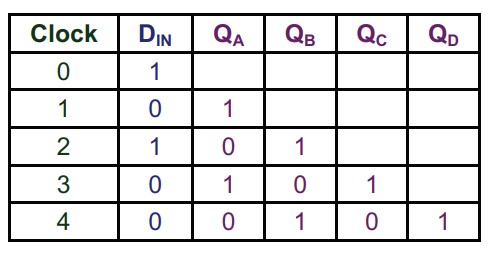
\includegraphics[width=\linewidth]{sipoTable.jpg}
The outputs $Q_A$ to $_D$ can be displayed on a timing diagram.
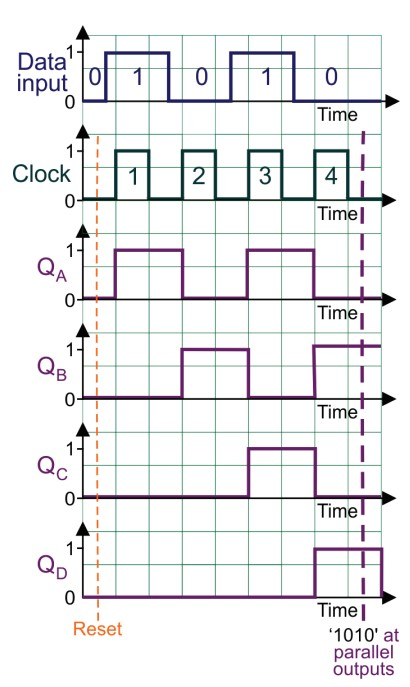
\includegraphics[width=\linewidth]{sipoTiming.jpg}

\section{Pulse Code Modulation}
The process of sampling analogue signals and converting them into binary codes is known as pulse code modulation (PCM). Many of the blocks in the block diagrams shown below are the same as in the Digital Audio Systems within Signal Conversion.
\subsection{Transmitter}
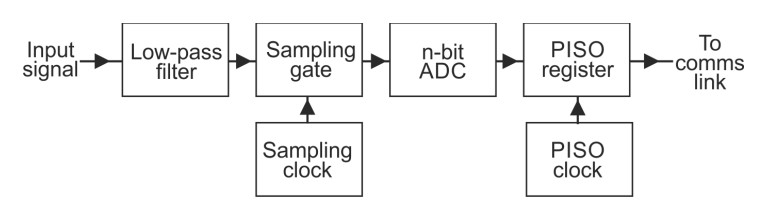
\includegraphics[width=\linewidth]{pcmTransmitterBlockDiagram.jpg}
\subsection{Receiver}
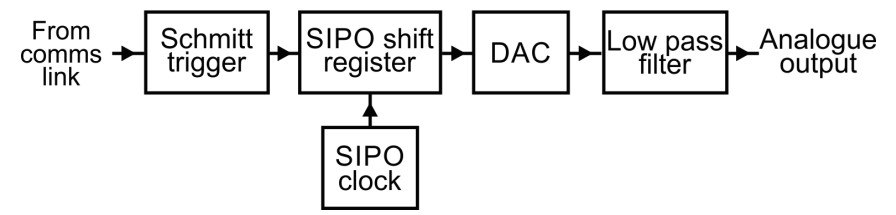
\includegraphics[width=\linewidth]{pcmReceiverBlockDiagram.jpg}
The Schmitt trigger is used to regenerate the signal. 

\section{Time Division Multiplexing}
Time Division Multiplexing is used to increase the capacity of a Pulse Code Modulation communications link. To illustrate how TDM works, a PCM telephone system will be used as an example.\\
In the UK, telephone bandwidth is limited to 3.4kHz, therefore $f_s = 6.8 kHz$. However, in reality we use 8kHz and a 12-bit ADC. \\
This means that
\begin{align*}
    f_s &= 8kHz\\
    \therefore T_s &= \frac{1}{8 \times 10 ^3} = 125 \mu s
\end{align*}
Where $T_s$ is the sampling period, which can be seen in the graph below.
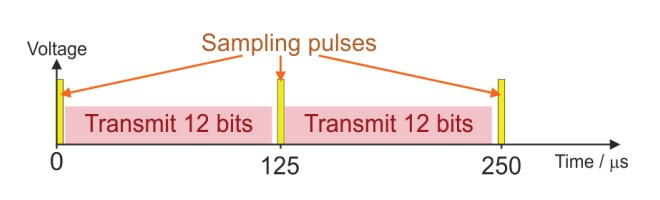
\includegraphics[width=\linewidth]{tdm1.jpg}
The frequency of the PISO shift register ($f_{PISO}$) can be calculated as follows:
\begin{align*}
    f_{PISO} &= 12 \times 8 = 96 kHz \\
    \therefore T_{PISO} &= \frac{1}{96 \times 10^3} = 10.4 \mu s
\end{align*}
Where $T_{PISO}$ is the time period of the PISO (time taken to set one bit).\\
If we now set $f_{PISO}$ to 1MHz, $T_{PISO} = 1 \mu s$ therefore the whole 12 bits take $12 \mu s$ to send.
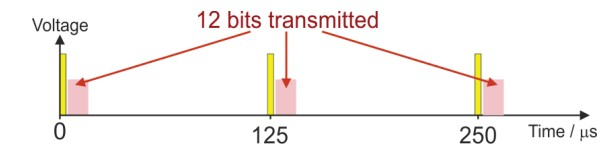
\includegraphics[width=\linewidth]{tdm2.jpg}
This means that we can now multiplex multiple signals together in the time domain. 
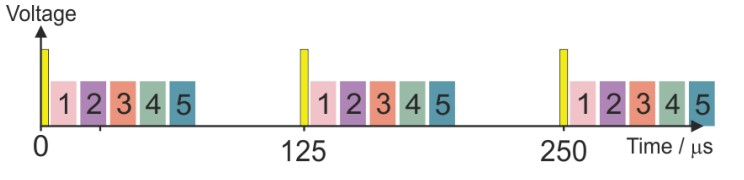
\includegraphics[width=\linewidth]{tdm3.jpg}
The maximum number of signals (channels) which can be multiplexed together can be calculated using the following formula.\\
$\displaystyle Max\ channels= \frac{sampling\ period}{num\ of\ bits \times PISO\ period}  $\\
Shown below is a block diagram of the entire TDM system.
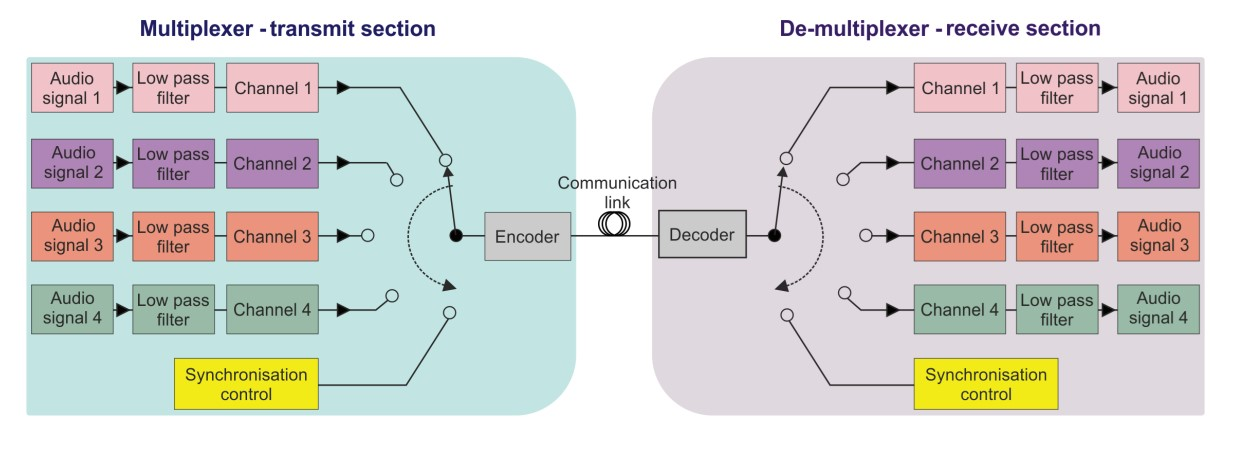
\includegraphics[width=\linewidth]{tdmFull.jpg}

\section{Pulse Width Modulation}
PWM represents the amplitude of the information signal with the width of the pulse train.
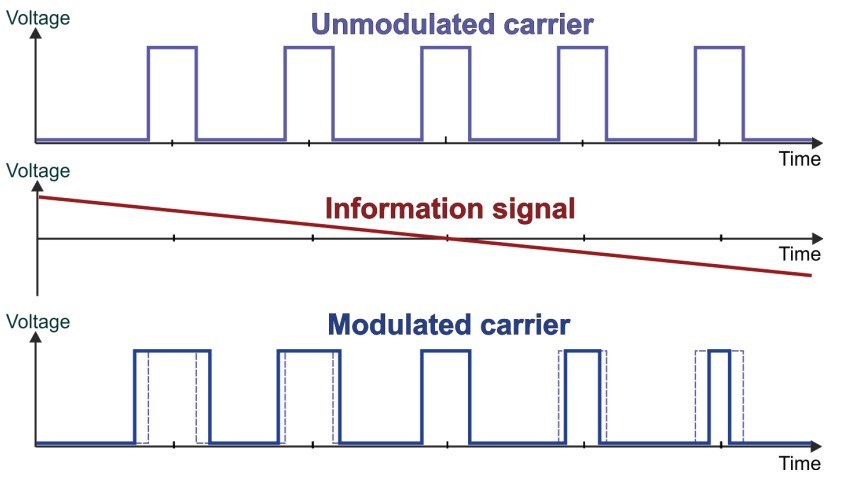
\includegraphics[width=\linewidth]{pwm.jpg}

\section{Pulse Position Modulation}
PPM represents the amplitude of the information signal with the position of the pulse train.
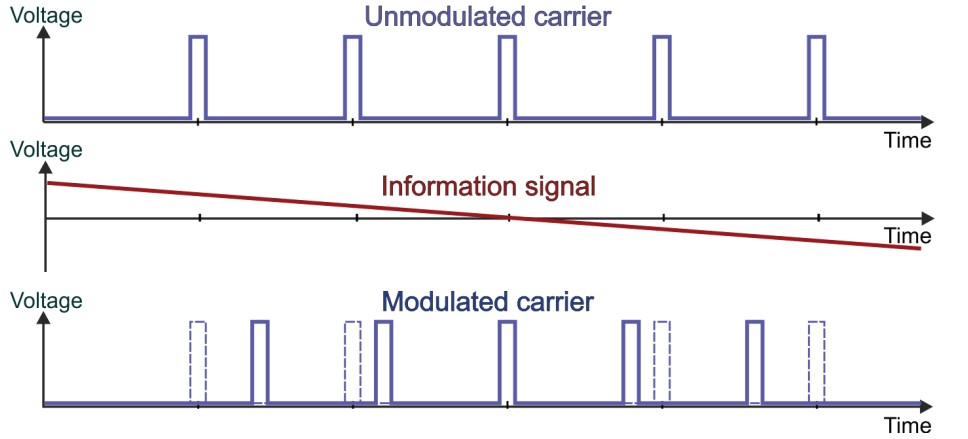
\includegraphics[width=\linewidth]{ppm.jpg}

\section{Schmitt Triggers}
When signals are transmitted, the signal quality can degrade. A schmitt trigger can be used to regenerate the signal and provide a clean wave.
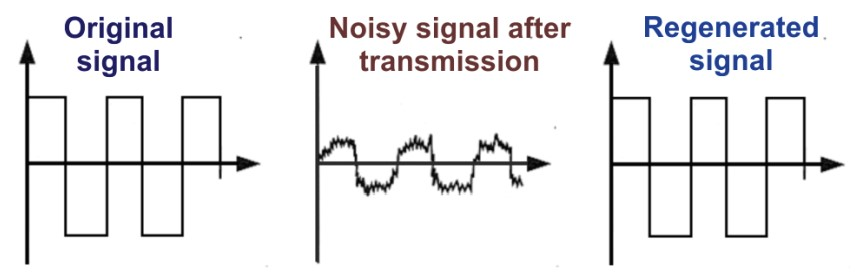
\includegraphics[width=\linewidth]{schmittPurpose.jpg}
\subsection{Non-Inverting Schmitt Trigger}
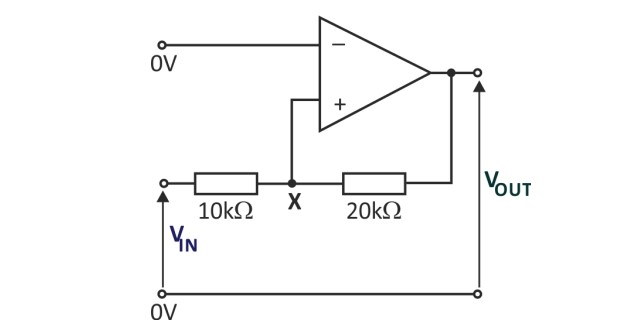
\includegraphics[width=\linewidth]{niSchmitt.jpg}
If $V_{OUT} = +V_{SAT}$, it stays in saturation as $V_X$ is positive. $V_{OUT}$ will flip when $V_{IN}$ goes negative, causing $V_X$ to be pulled negative.\\
If $V_{OUT} = -V_{SAT}$, stays in saturation as $V_X$ is negative. $V_{OUT}$ will flip when $V_{IN}$ becomes positive enough to pull $V_X$ positive.\\
The inverting input is $V_{REF}$.
\subsubsection{Calculating Thresholds}
In the exam, it is quite common to be asked to calculate a threshold for a schmitt trigger. First, assume that the comparator is initially in positive saturation and it will switch to negative saturation when $V_X < 0$; from this, calculate the lower threshold. Then assume the comparator is in negative saturation and calculate the upper threshold. If $V_{REF} = 0V$, the thresholds are symmetrical (eg, 6V \& -6V).

\end{document}

pwm
ppm
Schmitt